\chapter{Power Series Solution and Special Functions}
\section{Series Solution Method}
Series expansion is a  method of obtaining one solution of the linear, second-order, homogeneous ODE. The method, will always work, provided the point of expansion is no worse than a regular singular point. In physics this very gentle condition is almost always satisfied. 
A linear, second-order, homogeneous ODE can be written in the form
\begin{equation}
\frac{d^{2} y}{d x^{2}}+P(x) \frac{d y}{d x}+Q(x) y=0 \label{DE002}
\end{equation}
The most general solution of the equation \ref{DE002} may be written as,
\begin{equation}
y(x)=c_{1} y_{1}(x)+c_{2} y_{2}(x)
\end{equation}
But a physical problem may lead to a nonhomogeneous, linear, second-order ODE
\begin{equation}
\frac{d^{2} y}{d x^{2}}+P(x) \frac{d y}{d x}+Q(x) y=F(x)\label{DE003}
\end{equation}
Hence the most general solution to the equation \label{DE003} will be of the form,
\begin{equation}
y(x)=c_{1} y_{1}(x)+c_{2} y_{2}(x)+y_{p}(x)
\end{equation}
The constants $c_{1}$ and $c_{2}$ will eventually be fixed by boundary conditions.\\\\
There are two series solution method  for differential equation,
\begin{enumerate}
	\item \textbf{Simple series expansion method}
	\item \textbf{Frobenious Method}
\end{enumerate}
\subsection{Simple Power Series Expansion Method}
The simple series expansion method works for differential equations whose solutions are well-behaved at the expansion point $x = 0$.
We illustrate the method of series solution by solving the following simple equation (which you can easily solve by elementary methods also!).
\begin{align}
y^{\prime}&=2 x y\label{SP-05}
\intertext{We assume a solution of this differential equation in the form of a power series, namely}
y&=a_{0}+a_{1} x+a_{2} x^{2}+a_{3} x^{3}+\cdots+a_{n} x^{n}+\cdots\notag\\
&=\sum_{n=0}^{\infty} a_{n} x^{n}\label{SP-06}
\intertext{where the $a$ 's are to be found. Differentiating $(1.2)$ term by term, we get}
 y^{\prime} &=a_{1}+2 a_{2} x+3 a_{3} x^{2}+\cdots+n a_{n} x^{n-1}+\cdots \notag\\ &=\sum_{n=1}^{\infty} n a_{n} x^{n-1} \label{SP-07}
 \intertext{We substitute (\ref{SP-06}) and (\ref{DE007}) into the differential equation (\ref{SP-05}); we then have two power series equal to each other. Now the original differential equation is to be satisfied for all values of $x$, that is, $y^{\prime}$ and $2 x y$ are to be the same function of $x$. Since a given function has only one series expansion in powers of $x$ (see Chapter 1 , Section 11), the two series must be identical, that is, the coefficients of corresponding powers of $x$ must be equal. We get the following set of equations for the $a$ 's:}
 a_{1}&=0, \quad a_{2}=a_{0}, \quad a_{3}=\frac{2}{3} a_{1}=0, \quad a_{4}=\frac{1}{2} a_{0}
 \intertext{or in general:}
 n a_{n}&=2 a_{n-2}, \quad a_{n}= \begin{cases}0, & \text { odd } n, \\ \frac{2}{n} a_{n-2}, & \text { even } n .\end{cases}\\
\text{ Putting }n&=2 m\text{ (since only even terms appear in this series), we get}\notag\\
a_{2 m}&=\frac{2}{2 m} a_{2 m-2}=\frac{1}{m} a_{2 m-2}=\frac{1}{m} \frac{1}{m-1} a_{2 m-4}=\cdots=\frac{1}{m !} a_{0}
\intertext{Substituting these values of the coefficients into the assumed solution (\ref{SP-06}) gives the solution}
y&=a_{0}+a_{0} x^{2}+\frac{1}{2 !} a_{0} x^{4}+\cdots+\frac{1}{m !} a_{0} x^{2 m}+\cdots=a_{0} \sum_{m=0}^{\infty} \frac{x^{2 m}}{m !}
\end{align}
\subsection{Classical Linear Oscillator}
\begin{align}
\frac{d^{2} y}{d x^{2}}+\omega^{2} y&=0 \label{DE003}\\
\text{with known solutions} \ y&=\sin \omega x, \cos \omega x\\
\text{We try}\ y(x) &=x^{k}\left(a_{0}+a_{1} x+a_{2} x^{2}+a_{3} x^{3}+\cdots\right) \\
&=\sum_{\lambda=0}^{\infty} a_{\lambda} x^{k+\lambda}, \quad a_{0} \neq 0 \label{DE004}\\
\intertext{with the exponent $k$ and all the coefficients $a_{\lambda}$ still undetermined. Note that $k$ need not be an integer. By differentiating twice, we obtain}
\frac{d y}{d x} &=\sum_{\lambda=0}^{\infty} a_{\lambda}(k+\lambda) x^{k+\lambda-1} \\
\frac{d^{2} y}{d x^{2}} &=\sum_{\lambda=0}^{\infty} a_{\lambda}(k+\lambda)(k+\lambda-1) x^{k+\lambda-2}
\intertext{By substituting into equation.\ref{DE003}, we have}
\sum_{\lambda=0}^{\infty} a_{\lambda}(k+\lambda)(k+\lambda-1) x^{k+\lambda-2}+\omega^{2} \sum_{\lambda=0}^{\infty} a_{\lambda} x^{k+\lambda}&=0 \label{DE005}
\intertext{The coefficients of each power of $x$ on the left-hand side of equation.\ref{DE005} must vanish individually.The lowest power of $x$ appearing in equation.\ref{DE005} is $x^{k-2}$, for $\lambda=0$ in the first summation. The requirement that the coefficient vanish  yields,}
a_{0} k(k-1)&=0
\intertext{We had chosen $a_{0}$ as the coefficient of the lowest nonvanishing terms of the series \ref{DE004}, hence, by definition, $a_{0} \neq 0$. Therefore we have,}
k(k-1)&=0 \label{DE006}
\end{align}
\textbf{This equation, coming from the coefficient of the lowest power of $x$, we call the {indicial equation}.} The indicial equation and its roots are of critical importance to our analysis.
\\From equation.\ref{DE006}, \qquad $k=0 $ or $k=1$\\
The only way a power series can be zero is, it's coefficients must be equal to zero. But here the power of $x$ in the equation do not match up. The Coefficent of $x$ in the first term is,${k+\lambda-2} $ and for the second term it is,$k+\lambda$, to make them equal, we can replace $\lambda$ by $\lambda+2$ in the first term. Then we get,
\begin{align}
\sum_{\lambda=2}^{\infty} a_{\lambda+2}(k+\lambda+2)(k+\lambda+1) x^{k+\lambda}+\omega^{2} \sum_{\lambda=0}^{\infty} a_{\lambda} x^{k+\lambda}&=0\\
\sum_{\lambda=2}^{\infty} a_{\lambda+2}(k+\lambda+2)(k+\lambda+1) +\omega^{2} \sum_{\lambda=0}^{\infty} a_{\lambda} &=0
\intertext{Here the coefficients  are independent summations and $\lambda $ is a dummy index. Then we get,}
a_{\lambda+2}(k+\lambda+2)(k+\lambda+1) +\omega^{2} a_{\lambda} &=0\\
a_{\lambda+2}&=-a_{\lambda} \frac{\omega^{2}}{(k+\lambda+2)(k+\lambda+1)}\label{DE007}
\end{align}
For this example, if we start with $a_{0}$, Equation.\ref{DE007} leads to the even coefficients $a_{2}, a_{4}$, and so on, and ignores $a_{1}, a_{3}, a_{5}$, and so on. Since $a_{1}$ is arbitrary if $k=0$ and necessarily zero if $k=1$, 
$$
a_{3}=a_{5}=a_{7}=\cdots=0
$$
and all the odd-numbered coefficients vanish. The odd powers of $x$ will actually reappear when the second root of the indicial equation is used.
\begin{align}
a_{\lambda+2}&=-a_{\lambda} \frac{\omega^{2}}{(\lambda+2)(\lambda+1)}
\intertext{which leads to}
a_{2}&=-a_{0} \frac{\omega^{2}}{1 \cdot 2}=-\frac{\omega^{2}}{2 !} a_{0} \\
a_{4}&=-a_{2} \frac{\omega^{2}}{3 \cdot 4}=+\frac{\omega^{4}}{4 !} a_{0} \\
a_{6}&=-a_{4} \frac{\omega^{2}}{5 \cdot 6}=-\frac{\omega^{6}}{6 !} a_{0}, \quad \text { and so on. }
\intertext{By inspection (and mathematical induction),}
a_{2 n}&=(-1)^{n} \frac{\omega^{2 n}}{(2 n) !} a_{0}
\intertext{and our solution is}
y(x)_{k=0}&=a_{0}\left[1-\frac{(\omega x)^{2}}{2 !}+\frac{(\omega x)^{4}}{4 !}-\frac{(\omega x)^{6}}{6 !}+\cdots\right]\\&=a_{0} \cos \omega x\\
\intertext{If we choose the indicial equation root $k=1$ Equation.\ref{DE007}, the recurrence relation becomes}
a_{j+2}&=-a_{j} \frac{\omega^{2}}{(j+3)(j+2)}\\
\intertext{Substituting in $j=0,2,4$, successively, we obtain}
a_{2}=-a_{0} \frac{\omega^{2}}{2 \cdot 3}&=-\frac{\omega^{2}}{3 !} a_{0} \\
a_{4}=-a_{2} \frac{\omega^{2}}{4 \cdot 5}&=+\frac{\omega^{4}}{5 !} a_{0} \\
a_{6}=-a_{4} \frac{\omega^{2}}{6 \cdot 7}&=-\frac{\omega^{6}}{7 !} a_{0}, \quad \text { and so on. }
\intertext{Again, by inspection and mathematical induction,}
a_{2 n}&=(-1)^{n} \frac{\omega^{2 n}}{(2 n+1) !} a_{0}\\
\intertext{For this choice, $k=1$, we obtain}
y(x)_{k=1} &=a_{0} x\left[1-\frac{(\omega x)^{2}}{3 !}+\frac{(\omega x)^{4}}{5 !}-\frac{(\omega x)^{6}}{7 !}+\cdots\right] \\
&=\frac{a_{0}}{\omega}\left[(\omega x)-\frac{(\omega x)^{3}}{3 !}+\frac{(\omega x)^{5}}{5 !}-\frac{(\omega x)^{7}}{7 !}+\cdots\right] \\
&=\frac{a_{0}}{\omega} \sin \omega x
\end{align}
\subsubsection{Power Series Solution (About an Ordinary Point)}
Find the power series solution of $\left(1-x^{2}\right) y^{\prime \prime}-2 x y^{\prime}+2 y=0$ about $x=0$\\\\
Since $x=0$ is an ordinary point of the given differential equation, the solution can be written as
\begin{align*}
y&=\sum_{k=0}^{\infty} a_{k} x^{k} \\ \frac{d y}{d x}&=\sum_{k=0}^{\infty} k a_{k} x^{k-1} \\ \frac{d^{2} y}{d x^{2}}&=\sum_{k=0}^{\infty} a_{k} k(k-1) x^{k-2}
\intertext{Substituting these values in the given equation we get,}
\left(1-x^{2}\right) \sum_{k} a_{k} k(k-1) x^{k-2}&-2 x \sum_{k} a_{k}(k) x^{k-1}+2 \sum_{k} a_{k} x^{k}=0 \\
\sum_{k=2} a_{k} k(k-1) x^{k-2}&-\sum\left(k^{2}+k-2\right) a_{k} x^{k}=0
\intertext{now equating the coefficient of $x^{k}$ then}
(k+2)(k+1) a_{k+2}-\left(k^{2}+k-2\right) a_{k}&=0 \\a_{k+2}&=\frac{k-1}{(k+1)} a_{k}\\
\text{For} \ k&=0 \Rightarrow a_{2}=-a_{0} \\ k&=1 \Rightarrow a_{3}=0 \\
k&=2 \Rightarrow a_{4}=\frac{a_{2}}{3}=\frac{-a_{0}}{3}  \\ k&=3 \Rightarrow a_{5}=\frac{2}{4} a_{3}=0\\
\text{Therefore, solution}\ y&=a_{0}+a_{1} x+a_{2} x^{2}+\ldots \ldots\\&=a_{0}\left[1-x^{2}-\frac{x^{4}}{3} \ldots . .\right]+a_{1} x
\end{align*}
%\subsection{Frobenious Method}
%Even though the simple power series expansion method works for many functions there are some whose behaviour  precludes the simple series method like the Bessel's function. The need of Frobenious method  lies under the fact that, \textbf{any functions involving negative or fractional powers would not be amenable to power series solution method}. The Frobenious method extends the simple power series solution method to include negative and fractional powers, and it also allows a natural extension involving logarithm terms.\\
%The basic idea of the Frobenius method is to look for solutions of the form
%\begin{align*}
%y(x) &=a_{0} x^{\lambda}+a_{1} x^{\lambda+1}+a_{2} x^{\lambda+2}+a_{3} x^{\lambda+3}+\ldots \\
%&=x^{\lambda}\left(a_{0}+a_{1} x+a_{2} x^{2}+a_{3} x^{3}+\ldots\right) \\
%&=x^{\lambda} \sum_{k=0}^{\infty} a_{k} x^{k} \\
%&= \sum_{k=0}^{\infty} a_{k} x^{k+\lambda}
%\end{align*}
%The extension of the simple power series method is all in the factor $x^{\lambda}$. The power $c$ must now be determined, as well as the coefficients $a_{k}$. Since $\lambda$ may be negative, positive, and possibly non-integral, this extends considerably the range of functions which may be treated. Note that $a_{0}$ is the lowest non-zero coefficient, so by definition it cannot be zero.
\section{Singularity}
Consider differential equation,
\begin{equation}
\frac{d^2y}{dx^2} +P(x)\frac{dy}{dx}+Q(x)y=0
\end{equation}
\begin{enumerate}
	\item If $P(x)$ and $Q(x)$ remain finite at $x=x_0$ then it is ordinary point
	\item If either $P(x)/Q(x)$ or both tends to $\infty$ at $x=x_0$
	then it is singular point.
\end{enumerate}
\subsection{Kinds of singular points}
\begin{enumerate}
	\item \textbf{Regular singularity}\\\\
	IF $P(x), Q(x)\text{ diverges but } (x-x_0) P(x) \text{ and }(x-x_0)^2Q(x)$ remain finite at $x\rightarrow x_0$ then $x=x_0$ is called regular or non essencial singular points
	\item \textbf{Irregular singularity}\\\\
	$P(x), Q(x)$ diverges and either $(x-x_0)P(x)$ or $(x-x_0)^2Q(x)$ or both  remain infinite at $x\rightarrow x_0$ then $x=x_0$ is called irregular or essential singular points
\end{enumerate}
\textbf{Little bit review of Ordinary Differential Equations}
\begin{equation*}
\frac{d^2y }{dx^2}+P(x)\frac{dy}{dx}+Q(x)y=R(x)
\end{equation*}
Using Tailor series expansion method. If a function was continues and differentable you could express it as an infinite series of polynomial terms being added.
\begin{align*}
y(x)&=\sum\limits_{n=0}^{\infty}a_n(x-x_0)^n\\
y^\prime(x)&=\sum\limits_{n=0}^{\infty}na_n(x-x_0)^{n-1}\\
y^{\prime\prime}(x)&=\sum\limits_{n=0}^{\infty}n(n-1)a_n(x-x_0)^{n-2}      \intertext{Plugging this value into the differential equation we can express as}
\sum\limits_{n=0}^{\infty}n(a-1)a_n(x-x_0)^{n-2}&+\sum\limits_{n=0}^{\infty}na_n(x-x_0)^{n-1}P(x)+Q(x)\sum\limits_{n=0}^{\infty}a_n(x-x_0)^n=R(x)
\intertext{$P(x),Q(x)$ and $R(x)$ are also functions of $x$. It's also possible to express them as power series} 
P(x)=\sum\limits_{n=0}^{\infty}b_n(x-x_0)^n\quad Q(x)&=\sum\limits_{n=0}^{\infty}c_n(x-x_0)^n,R(x)=\sum\limits_{n=0}^{\infty}d_n(x-x_0)^n\\
\intertext{$\sum\limits_{n=0}^{\infty}n(n-1)a_n(x-x_0)^{n-2}+\sum\limits_{n=0}^{\infty}b_n(x-x_0)^n \sum\limits_{n=0}^{\infty}na_n(x-x_0)^{n-1}+\sum\limits_{n=0}^{\infty}c_n(x-x_0)^n  \sum\limits_{n=0}^{\infty}a_n(x-x_0)^n    $}
&=\sum\limits_{n=0}^{\infty}d_n(x-x_0)^n
\end{align*}
 To find $a_n$,
 we should properly expand $P(x),Q(x)$ and $R(x)$ abt $x=x_0$ If any one of function is undefined at $x_0$ then we would not be able to do it.\\\\
\textbf{Example:}\\
\begin{equation*}
\frac{d^2y}{dx^2}-4y=0, \ y(x)=\sum\limits_{n=0}^{\infty}a_n(x-x_0)^n
\end{equation*}

It will always continuos and differentiable about $x_0=0$, So we will have a valid tylor series expansion about this point and we can proceed with a power series expansion method.
\begin{align*}
y(x)&=\sum\limits_{n=0}^{\infty}a_nx^n\qquad\ y^\prime(x)=\sum\limits_{n=0}^{\infty}na_n x^{n-1}\qquad
y^{\prime\prime}(x)=\sum\limits_{n=0}^{\infty}n(n-1)a_nx^{n-2}
\end{align*}
substituting into differential equation
\begin{align*}
\sum\limits_{n=0}^{\infty}n(n-1)a_nx^{n-2}-4\sum\limits_{n=0}^{\infty}a_n x^n&=0\\
\sum\limits_{n=0}^{\infty}n(n-1)a_n x^{n-2}-4 \sum\limits_{n=2}^{\infty}a_{n-2}x^{n-2}=0&\\\text{ expanding  first two terms of the }
\sum\limits_{n=0}^{\infty}n(n-1)a_n x^{n-2} &\text{we can express as }\\
\sum\limits_{n=2}^{\infty}n(n-1)a_nx^{n-2}-4\sum\limits_{n=2}^{\infty}a_{n-2}x^{n-2}&=0\\
\text{	combining }\sum\limits_{n=2}^{\infty}\left[n(n-1)a_n-4a_{n-2} \right] x^{n-2}&=0\\
\text{	since  RHS }=0 \text{}\\
\implies n(n-1)a_n-4a_{n-2}&=0
\intertext{If relates the $n^{th}$ term in the sequence of coefficient to terms that occured  previously in that sequence}
a_n=\frac{4a_{n-2}}{n(n-1)}&
\end{align*} 
$n^{th}$ coefficient is related to two terms back in the sequence\\
we have two solutions for differential equations, even part and odd part
\begin{align*}
\intertext{\textbf{Case$\ 1$}\quad $\rightarrow n=$\text{Even}}
a_2&=\frac{4a_0}{2.1}\quad
a_4=\frac{4a_2}{4.3}\\
&=\frac{4.4 \ a_0}{4.3\  2.1}\\
&\text{A pattern is developing}\\
a_4&=\frac{2^4\ a_0}{4!}\quad \text{it follows that}\\
a_n&=\frac{2^2 a_0}{n!}\\
&\text{Since a is even}\\
a_{2k}&=\frac{2^{2k\ a_0}}{(2k)!}\\
&\text{any even number can represent as multiple of $2$}\\
\text{here }&k=0,1,2,3 
\intertext{\textbf{Case$\ 2$}\quad $\rightarrow n=$\text{Odd}}
a_3&=\frac{4\ a_1}{3.2.1},\ a_5=\frac{4\ a_3}{5.4}=\frac{4.4.a_1}{5.4.3.2.1}\\
a_5&=\frac{2^4\ a_1}{5!}\quad \therefore a_n=\frac{2^{n-1}\ a_1}{n!}\\
&\text{It can be expressed as}\\
a_{2k+1}&=\frac{2^{2k}\ a_1}{(2k+1)!}\\
\intertext{ substituting in $y(x)=\sum\limits_{n=0}^{\infty}a_nx^n$ and expanding,}
&=a_0+a_1x+a_2x^2+a_3x^3+\dots a_{2k}x^{2k}+a_{2k+1}x^{2k+1}+\dots\\
&=a_0+a_1x+\frac{2^2\ a_0}{2!}x^2+\frac{2^2\ a_1}{3!}x^3+\dots+\frac{2^{2k}\ a_0}{(2k)!}+\frac{2^{2k}\ a_1}{(2k+1)!}+\dots\\
&\text{ By seperating even and odd solutions we can express as}\\
y(x)&=\sum\limits_{k=0}^{\infty}\frac{2^{2k}\ a_0}{(2k)!}x^{2k}+\sum\limits_{k=0}^{\infty}\frac{2^{2k}\ a_1}{(2k+1)!}x^{2k+1}
\end{align*}
Here we discuss series solution and how to use power series to solve differential equations.Now we can check how to use this methode to solve one of the important problems in maths and physics, The legendre diffrential equation problem.
\section{Legendre Function}
\begin{align*}
(1-x^2)\frac{d^2y}{dx^2}&-2x\frac{dy}{dx}+k(k+1)y=0\\
&\text{to expand it in } 
x_0=0\\
\frac{d^2y}{dx^2}&+\frac{P(x)dy}{dx}+Q(x)y=R(x)\text{(General form)}
\intertext{To compare our equation with General form we can express as }
\frac{d^2y}{dx^2}&-\frac{2x}{(1-x^2)}\frac{dy}{dx}+\frac{k(k+1)}{1-x^2}y=0\\\
&\text{ $P(x),Q(x)$ and $R(x)$ are all defined at $x=0$, So it is possible for regular series solution at $x_0=0$}\\
\end{align*}
\begin{align*}
y(x)&=\sum\limits_{n=0}^{\infty}a_nx^n\\
y^{\prime}(x)&=\sum\limits_{n=0}^{\infty}na_nx^{n-1}\\
y^{\prime\prime}(x)&=\sum\limits_{n=0}^{\infty}n(n-1)a_nx^{n-2}\\
(1-x^2)\sum\limits_{n=0}^{\infty}n(n-1)&a_nx^{n-2}-2x\sum\limits_{n=0}^{\infty}na_nx^{n-1}+k(k+1)\sum\limits_{n=0}^{\infty}a_nx^{n}=0\\
\sum\limits_{n=0}^{\infty}n(n-1)&a_nx^{n-2}-\sum\limits_{n=0}^{\infty}n(n-1)a_nx^{n}-\sum\limits_{n=0}^{\infty}2na_nx^n+\sum\limits_{n=0}^{\infty}k(k+1)a_nx^{n}=0\\
\intertext{To combain the terms, we have to make power of $x$ and limits same, after necessary steps we can express as}
\sum\limits_{n=0}^{\infty}&a_{n+2}(n+2)(n+1)x^n-\sum\limits_{n=0}^{\infty}n(n-1)a_nx^n-\sum\limits_{n=0}^{\infty}2na_nx^n+\sum\limits_{n=0}^{\infty}k(k+1)a_nx^n=0\\
\sum\limits_{n=0}^{\infty}&\left[ a_{n+2}(n+2)(n+1)-a_nn(n-1)-2na_n+k(k+1)a_n\right] x^n=0\\
a_{n+2}&(n+2)(n+1)-a_nn(n-1)-2na_n+k(k+1)a_n=0\\
a_{n+2}&=\frac{a_{n}[(n-k)(n+k)+(n-k)] }{(n+2)(n+1)}=\frac{a_{n}(n-k)(n+k+1)}{(n+2)(n+1)}
\intertext{\textbf{Case$\ 1$}\quad $\rightarrow n=$\text{Even}}
a_2&=\frac{a_{0} \cdot(-k)(x+1)}{2 \cdot 1}\\
a_4&=\frac{a_{2}(2-k)(3+k)}{4\cdot 3}=\frac{(k-2) k(k+1)(k+3) a_{0}}{4!}
\intertext{\textbf{Case$\ 2$}\quad $\rightarrow n=$\text{Odd}}
a_3&=\frac{a_{1}(1-k)(2+k)}{3\cdot2}\\
a_5&=\frac{9_{3}(3-k)(4+k)}{5.4}=\frac{a_{1}(k-3)(k-1)(k+2)(k+4)}{5!}
\end{align*}
1.\quad What if $k=1$ 
\begin{align*}
 a_3&=0\\
\text{all coefficients come later on }a_3&=0 
\text{ since they depend on }a_3\\
\text{so solution},\ 
&y_{odd}=a_1x=a_1P_1(x)\\
P_1(x)\text{ is just a function of $x$}
\text{, even series }&\text{doesnot terminate}\end{align*}
2.\quad What if $k=2$
\begin{align*}
a_2&=a_{0} \frac{(-2)(3)}{2}=-3 a_{0}, \ a_{4}=0\\
y_{\text {even }}&=a_{0}-3 a_{0} x^{2}=a_{0}\left(1-3 x^{2}\right)\\
&=\cdot 5\left(3 x^{2}-1\right)=P_{2}(x) \text{ for }a_0=\frac{-1}{2}\\
\text{for }k&=2,\text{ odd series doesnot terminate}\\
k&=3\\
y_ {odd} &=-\frac{5}{3} a_1 x^{3}+a_{1} x\\
&=\frac{1}{2}\left(5 x^{3}-3 x\right)=P_{3}(x)\text{ for }a_{1}=-3 / 2\\
\text{even series }&\text{doesnot terminate for odd value of $k$}
\end{align*}
we can repeat this for different value of $k$, for even $k$, even series terminates and 
for odd $k$, odd series terminates\\
$P_1, P_2, P_3$ they result from series terminating are not like just other polynomial they are special polynomial.\\
$P_1, P_2, P_3$ are called legendre polynomials, they are solutions to legendre diffrential equations they come up in electromagnetism and quantum mechanics. Bunch of techniques already developed to calculate legendre polynomials more easily and one of these techniques is rodrigues formula
$P_{k}(x)=\frac{1}{2^{k} k !} \frac{d^{k}}{d x^{k}}\left[\left(x^{2}-1\right)^{k}\right]$\\
\section{Frobenius Method}
For power series solution, \  $y^{\prime\prime}+P(x)y^\prime +Q(x)y=R(x)$\ only have valid series solution about $x=x_0$ if $P(x),Q(x)$ and $R(x)$ have valid tylor series at $x_0$. We want them to be continues and differentiable at that point. What if $P(x),Q(x),R(x)$ did not have valid tylor expansions about $x_0$ but still wanted series solution about $x_0$? We could do it by using a slightly modified version. All is to do include $r$ to the regular series solution. $r$ is a real number. This is called Frobenius method. Using Frobenius method still can have  solution to be power series solution at singular point. But point has to be regular singular point. 
\begin{align*}
&2(x-1)^2y^{\prime\prime}-(x-1)y^\prime+y=0\\
&2 y^{\prime \prime}-\frac{1}{(x-1)} y^{\prime}+\frac{1}{(x-1)^{2}} y=0
\intertext{x=1 makes this undefined, but point 1 is a regular singular point. So we can express using frobenius method as}
&y=\sum_{k=0}^{\infty} a_{k}(x-1)^{k+\lambda}\\
&y^{\prime}=\sum_{k=0}^{\infty}(n+\lambda) a_{k}(x-1)^{k+\lambda-1}
\quad y^{\prime \prime}=\sum_{k=0}^{\infty}(k+\lambda-1)(k+\lambda) a_{k}(x-1)^{k+\lambda-2}\\
&2 \sum_{k=0}^{\infty}(k+\lambda-1)(k+\lambda) a_{k}(x-1)^{k+\lambda-2}-\frac{1}{x-1}
\sum_{k=0}^{\infty}(k+\lambda) a_{k}(x-1)^{k+\lambda-1}+\frac{1}{(x-1)^{2}}\sum_{k=0}^{\infty} a_{k}(x-1)^{k+\lambda}=0\\
&2 \sum_{k=0}^{\infty}(k+\lambda-1)(k+\lambda) a_{k}(x-1)^{k+\lambda-2}-
\sum_{k=0}^{\infty}(k+\lambda) a_{k}(x-1)^{k+\lambda-2}+\sum_{k=0}^{\infty} a_{k}(x-1)^{k+\lambda-2}=0\\
&\sum_{k=0}^{\infty}\left[2(k+\lambda)(k+\lambda-1) a_{k}\right.\left.-(k+\lambda) a_{k}+a_{k}\right](x-1)^{k+\lambda-2}=0
\intertext{expanding few terms}
&\left[ 2 \lambda(\lambda-1)-\lambda+1\right] a_0(x-1)^{\lambda-2}+[2 \lambda(\lambda+1)-(\lambda+1)+1]a_1(x-1)^{\lambda-1}+...+=0\\
\intertext{equating coefficients of $(x-1)^{\lambda-2}$}
&2 \lambda^{2}-3 \lambda+1=0\\
\intertext{This is a quadratic equation and we call it as indicial equation.}
&\lambda_{1}=1 \quad \lambda_{2}=0.5
\end{align*}

$\therefore$ For equality to hold $a_1,a_2.....a_k,..=0$, what does this mean for final answer?\\
$y=\sum_{k=0}^{\infty} a_{k}(x-1)^{k+\lambda}=a_{0}(x-1)^{\lambda}$only first term correspond to $k=0$ is in the final expression, because of two vaues of $r$. \\ $y_1=a_{0}(x-1), y_{2}=a_{0}(x-1)^{.5}$.\\ General solution is : $y=c_{1}(x-1)+c_{2} \sqrt{x-1}$
\section{Bessel Function}
Bessel’s equation in the usual standard form is,
\begin{equation}
x^{2} \frac{d^{2} y}{d x^{2}}+x \frac{d y}{d x}+\left(x^{2}-n^{2}\right) y=0 \label{Bessel 1}
\end{equation}
Where $n$ is a constant (not necessarily an integer) called the order of the Bessel function $'y'$ which is the solution of equation.\ref{Bessel 1}. $x=0$ is a regular singular point of the Bessel differential equation.

\subsection{The solution of Bessel's function}
\begin{align*}
x^{2} y^{\prime\prime }+x y^\prime+\left(x^{2}-n^{2}\right) y&=0
\intertext{ $x_0=0$ is a regular singular point, so we can expand about $x_0=0$ using Frobenius method}
y=\sum_{k=0}^{\infty} a_{k} x^{k=\lambda}\quad y^{\prime}&=\sum_{k=0}^{\infty}(k=\lambda) a_{k} x^{k=\lambda-1}\quad y^{\prime \prime}=\sum_{k=0}^{\infty}(k=\lambda)(k=\lambda-1) a_{k}x^{k=\lambda-2}\\
\sum_{k=0}^{\infty}(k=\lambda)(k=\lambda-1) a_{k} x^{k=\lambda-2} &+\frac{1}{x} \sum_{k=0}^{\infty}(k=\lambda) a_{k}x^{k=\lambda-1}+\left(1-\frac{n^{2}}{x^{2}}\right) \sum_{k=0}^{\infty} a_{k} x^{k=\lambda}=0\\
\sum_{k=0}^{\infty}(k=\lambda)(k=\lambda-1) a_{k} x^{k=\lambda-2} &+\sum_{k=0}^{\infty}(k=\lambda) a_{k} x^{k=\lambda-2}+\sum_{n=0}^{\infty} a_{k} x^{k=\lambda}-n^{2}\sum_{k=0}^{\infty} a_{k}x^{k=\lambda-2} =0\\
\sum_{k=0}^{\infty}(k=\lambda)(k=\lambda-1) a_{k} x^{k=\lambda-2} &+\sum_{k=0}^{\infty}(k=\lambda) a_{k} x^{k=\lambda-2}+ \sum_{k=2}^{\infty} a_{k-2} x^{k=\lambda-2}-n^{2}\sum_{k=0}^{\infty} a_{k}x^{k=\lambda-2} =0\\
\sum_{k=2}^{\infty}(k=\lambda)(k=\lambda-1) a_{n} x^{k=\lambda-2}&+\sum_{k=2}^{\infty}(k=\lambda) a_{k} x^{k=\lambda-2}+\sum_{k=2}^{\infty}a_{k-2}x^{k=\lambda-2}-n^{2} \sum_{k=2}^{\infty} a_{k}  x^{k=\lambda-2}\\
+\lambda(\lambda-1) a_{0} x^{\lambda-2}+\lambda(\lambda+1) a_{1} x^{\lambda-1}&+\lambda a_{0} x^{\lambda-2}+(\lambda+1) a_{1} x^{\lambda-1}-n^2{a_{0}} x^{\lambda-2}-n^{2} a_1 x^{\lambda-1}=0
\intertext{ right hand side is 0, so each term of left hand side should be equal to 0 and we can express like this}
\text{for} x^{\lambda-2}, \lambda(\lambda-1) a_{0}+\lambda a_{0}-n^{2} a_{0}&=0, \text{we want }a_{0} \neq 0 \text{, so we can write as,}\\
\lambda(\lambda-1)+\lambda-n^{2}=0\quad \lambda^{2}-n^{2}&=0 \quad \lambda=\pm n
\text{,this is our indicial equations}
\intertext{Plugging the values of $\lambda$ in   $ x^{\lambda-1}$We can show  $a_{1}=0$ , and what left with the equation is} \\
\sum_{k=2}^{\infty}(k=\lambda)(k=\lambda-1) a_{k} x^{k=\lambda-2}&+\sum_{n=2}^{\infty}(k=\lambda) a_{k} x^{k=\lambda-2}+\sum_{k=2}^{\infty}a_{k-2}x^{k=\lambda-2}-n^{2} \sum_{k=2}^{\infty} a_{k}  x^{k=\lambda-2}=0\\
\sum_{k=2}^{\infty}(((k=\lambda)(k+ \lambda-1)&+(k=\lambda) n^2) a_{k}+\left.a_{k-2}\right) x^{k=\lambda-2}=0\\
\left[(k=\lambda)(k=\lambda-1)+(k=\lambda)-n^{2}\right] &a_{k}+a_{k-2}=0\\
a_{k}&=\frac{-a_{k-2}}{\left[(k=\lambda)^{2}-n^{2}\right]}\\
\text{substitute }\lambda_1&=n\\
a_{k}=\frac{-a_{k-2}}{k(k+2 n)}\implies &\text{recursion}\\
\text{since }a_1 =0, \ &
a_{3},\  a_{5}, \ a_{7},....=0
\intertext{For even intiger coefficients, $k=2r$}
a_{2 r}&=-\frac{a_{2 r-2}}{4 r(r+n)}\\
a_{2}&=\frac{-a_{0}}{4 \cdot 1 (1+n)}\\a_{4}&=-\frac{-a_{2}}{4 \cdot 2(2+n)}=\frac{(-1)^{2} a_{0}}{4^{2}(2 \cdot 1)(2+n)(1+n)}\\
\therefore a_{2 r}&=\frac{(-1)^{r}}{4{r}}\frac{a_{0}}{r !(n+r) \cdots(n+1)}\\
y_{1}&=x^{n}\sum_{r=0}^{\infty} \frac{(-1)^{r}}{4 r}\frac{a_{0}}{r !(n+r) . .(n+1)} x^{2 r}
\end{align*}
For particular value of $a_0$ this solution is given a special name, $ J_n(x)$, Bessel function of $I$ kind and $n$ is order of Bessel function.
The solution of Bessel's function, $J_{n}(x)$ is defined to be a Bessel function of the first kind, of integral order $r$.
\begin{align}
\mathrm{J}_{\mathrm{n}}(\mathrm{x})&=y=a_{0} \sum_{r=0}^{\infty} \frac{(-1)^{r}}{r !(n+r) !}\left(\frac{x}{2}\right)^{n+2 r}\label{Bessel 2} \\ \text { Where } \mathrm{a}_{0}&=\frac{1}{2^{n} \Gamma (n+1)} \notag\\
\mathrm{n}=0 \quad \Rightarrow \quad \mathrm{J}_{0}(\mathrm{x})&=\sum_{r=0}^{\infty} \frac{(-1)^{r}}{(r !)^{2}}\left(\frac{x}{2}\right)^{2 r}=1-\frac{x^{2}}{2^{2}}+\frac{x^{4}}{2^{2} \cdot 4^{2}}-\frac{x^{6}}{2^{2} \cdot 4^{2} \cdot 6^{2}}+\ldots . .\\
\mathrm{n}=1 \quad \Rightarrow \quad \mathrm{J}_{1}(x)&=\frac{x}{2}-\frac{x^{3}}{2^{2} 4}+\frac{x^{5}}{2^{2} \cdot 4^{2} \cdot 6}-\ldots .
\end{align}
\begin{figure}[H]
	\centering
	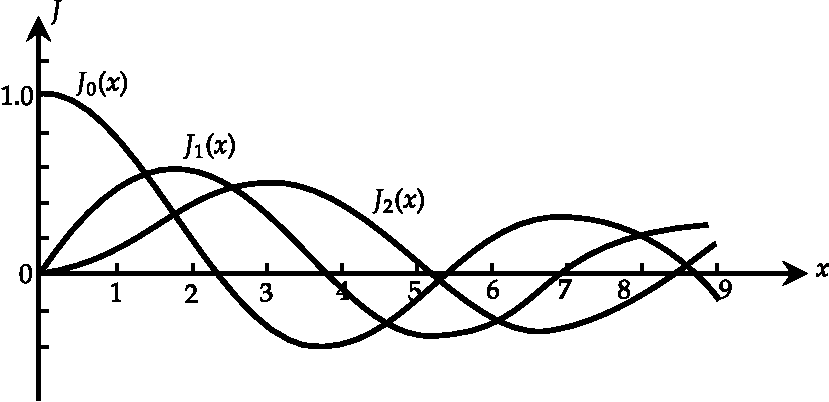
\includegraphics[height=4cm,width=7cm]{SF-03}
\end{figure}
\subsubsection{The second solution of Bessel's function}
We have found just one of the two solutions of Bessel’s equation, that is, the one
when $n>0$; we must next find the solution when $n<0$.  We can just replace $n$ by $-n$ in equation.\ref{Bessel 2}. 
The solution in $-n$ is usually written as $J_{-n}(x)$
\begin{equation}
J_{-n}(x)=\sum_{r=0}^{\infty} \frac{(-1)^{r}}{r !(r-n) !}\left(\frac{x}{2}\right)^{2 r-n} .
\end{equation}
And, 
\begin{equation}
J_{-n}(x)=(-1)^{n} J_{n}(x) \quad \text { for integral } n
\end{equation}
\subsubsection{Properties of Bessel's function.}
\begin{enumerate}
	\item Bessel functions are oscillatory function with varying period and decreasing amplitude.
	\item $J_{n}(x)$ is an even function when $n$ is even and $J_{n}(x)$ is an odd function when $n$ is odd.
	\item $\mathrm{J}_{0}(\mathrm{x})$ has nodes at $x=2.408,5.5201$......and $J_{1}(x)$ has nodes at $x=3.8317,7.015$.......
\end{enumerate}
\begin{note}$\left. \right. $\ The Bessel's functions for $n=\pm \frac{1}{2}$,
	\begin{align*}
	J_{1 / 2}(x)&=\sqrt{\frac{2}{\pi x}} \sin x \\ J_{-1 / 2}(x)&=\sqrt{\frac{2}{\pi x}} \cos x
	\end{align*}
\end{note}

\subsection{Generating function of Bessel's function:}
\begin{align*}
e^{\frac{x}{2}\left(z-\frac{1}{z}\right)}=\sum_{n=-\infty}^{\infty} z^{n} J_{n}(x)
\intertext{The coefficient of $z^{n}$ in the expansion of the generating tünction is the Bessel function of order $1 .$}
\end{align*}
\subsection{Orthogonal condition of Bessel Function:}
\begin{align*}
\int_{0}^{1} x_{n} \cdot(\alpha x) J_{n}(\beta x) d x=\frac{\delta_{\alpha \beta}}{2} \cdot\left[J_{n+1}(\alpha)\right]^{2}
\end{align*}
\subsection{Recurrencé relations for $J_{n}(x)$ :}
\begin{enumerate}
	\item $\frac{d}{d x}\left[x^{n} J_{n}(x)\right]=x^{n} J_{n-1}(x)$
	\item $\frac{d}{d x}\left[x^{-n} J_{n}(x)\right]=-x^{-n} J_{n+1}(x)$
	\item $J_{n-1}(x)+J_{n+1}(x)=\frac{2 n}{x} J_{n}(x)$
	\item $J_{n-1}(x)-J_{n+1}(x)=2 J_{n}^{\prime}(x)$
	\item $J_{n}^{\prime}(x)=-\frac{n}{x} J_{n}(x)+J_{n-1}(x)=\frac{n}{x} J_{n}(x)-J_{n+1}(x)$
\end{enumerate}

\begin{exercise}
	Show that $\sqrt{\frac{\pi x}{2}} J_{3 / 2}(x)=\frac{\sin x}{x}-\cos x$
\end{exercise}
\begin{answer}
	\begin{align*}
	\text{Using recurrence relation, }2 n J_{n}&=x\left[J_{n+1}+J_{n-1}\right]\\
	\text{putting}\mathrm{n}&=1 / 2,\text{ we get, }J_{1 / 2}=x\left[J_{3 / 2}+J_{-1 / 2}\right]\\
	x J_{3 / 2}&=J_{1 / 2}-x J_{-1 / 2} \\ \sqrt{\frac{\pi x}{2}} J_{3 / 2}&=\frac{\sin x}{x}-\cos x \text { (using the expressions of } J_{1 / 2} \& J_{-1 / 2} \text { ) }
	\end{align*}
\end{answer}
\section{Legendre Differential Equation}
\subsection{Rodrigue's Formula for Legendre's Polynomial $P_{n}(x)$ :}
\begin{align*}
\text { Legendre polynomial of order ' } n \text { ' : } P_{n}(x)&=\frac{1}{2^{n} n !} \frac{d^{n}}{d x^{n}}\left(x^{2}-1\right)^{n}\\
P_{0}(x)=1 ; \quad P_{1}(x)=x ; \quad P_{2}(x)&=\frac{1}{2}\left(3 x^{2}-1\right) ; \quad P_{3}(x)=\frac{1}{2}\left(5 x^{3}-3 x\right)
\end{align*}
\begin{figure}[H]
	\centering
	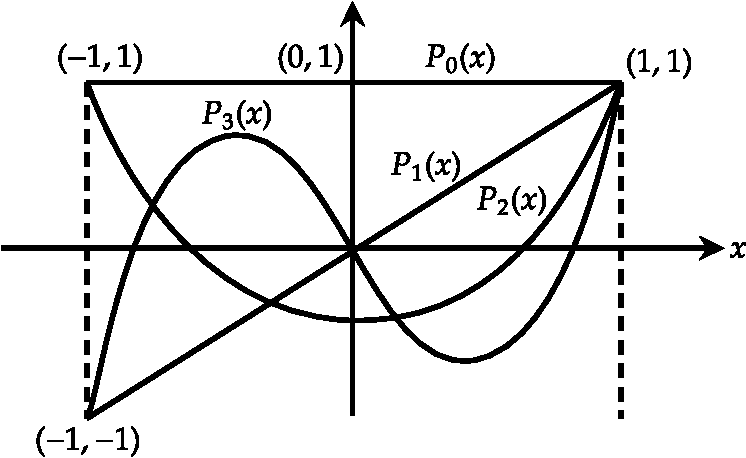
\includegraphics[height=3.8cm,width=6cm]{SF-02}
\end{figure}
\subsection{Properties of Legendre's Polynomial}
\begin{enumerate}
	\item $P_{n}(1)=1$
	\item $P_{n}(-1)=(-1)^{n}$
	\item $\left. \right.$\ $\begin{aligned}
	P_{n}(x)&=\text { even function, if } \mathrm{n}=\text { even }\\
	        &=\text { odd function, if } \mathrm{n}=\text { odd }
	\end{aligned}$
	\item $P_{n}(-x)=(-1)^{n} P_{n}(x)$
\end{enumerate}

\subsection{Generating function of Legendre's polynomial:}
$\left(1-2 x z+z^{2}\right)^{-1 / 2}$ is the generating function for legendre's polynomials i.e. $$\left(1-2 x z+z^{2}\right)^{-1 / 2}=\sum_{n=0}^{\infty} z^{n} P_{n}(x)$$
The co-efficient of $z^{n}$ in the exapansion of the generating function is the Legendre's polynomial of order $n$.
\subsection{Orthogonal properties of Legendre's polynomial:}
\begin{align*}
\int_{-1}^{+1} P_{m}(x) P_{n}(x) d x=\frac{2}{2 n+1} \delta_{m n} \text { where } \delta_{m n}=\text { Kronecker delta }&=1 \quad \text { if } \mathrm{m}=\mathrm{n}\\
&=0 \quad \text { if } m \neq n
\end{align*}
\subsection{Recurrence relations for $P_{n}(x)$ }
\begin{enumerate}
	\item $n P_{n}=(2 n-1) x P_{n-1}-(n-1) P_{n-2}$
	\item $n P_{n}=x P_{n}^{\prime}-P_{n-1}^{\prime}$
	\item $(2 n+1) P_{n}=P_{n+1}^{\prime}-P_{n-1}^{\prime}$
	\item $(n+1) P_{n}=P_{n+1}^{\prime}-x P_{n}^{\prime}$
	\item $\left(1-x^{2}\right) P_{n}^{\prime}=n\left(P_{n-1}-x P_{n}\right)$
	\item $\left(1-x^{2}\right) P_{n}^{\prime}=(n+1)\left(x P_{n}-P_{n+1}\right)$
\end{enumerate}

\begin{exercise}
	Express $4 x^{3}+6 x^{2}+7 x+2$ in terms of Legendre Polynomials.
\end{exercise}
\begin{answer}
	\begin{align*}
	\text { Let, } 4 x^{3}+6 x^{2}+7 x+2&=a_{3} P_{3}(x)+a_{2} P_{2}(x)+a_{1} P_{1}(x)+a_{0} P_{0}(x)\\
	&=\frac{a_{3}}{2}\left(5 x^{3}-3 x\right)+\frac{a_{2}}{2}\left(3 x^{2}-1\right)+a_{1} x+a_{0}\\
	\text { Comparing the co-efficient of } &\mathrm{x}^{3}: \frac{5 a_{3}}{2}=4 \Rightarrow a_{3}=\frac{8}{5}\\
	\text { Comparing the co-efficient of }& x^{2}: \frac{3 a_{2}}{2}=6 \Rightarrow a_{2}=4\\
	\text { Comparing the co-efficient of }& x^{1}:-\frac{3 a_{3}}{2}+a_{1}=7 \Rightarrow a_{1}=\frac{47}{5}\\
	\text { Comparing the co-efficient of }& \mathrm{x}^{0}:-\frac{a_{2}}{2}+a_{0}=2 \Rightarrow a_{0}=4\\
	\text { Therefore, } 4 x^{3}+6 x^{2}+7 x+2&=\frac{8}{5} P_{3}(x)+4 P_{2}(x)+\frac{47}{5} P_{1}(x)+4 P_{0}(x)
	\end{align*}
\end{answer}
\begin{exercise}
	Show that, $\int_{-1}^{1} x^{2} P_{n+1} P_{n-1} d x=\frac{2 n(n+1)}{(2 n-1)(2 n+1)(2 n+3)}$
\end{exercise}
\begin{answer}
	\begin{align*}
	\text{Using the relation: }&(2 n+1) x P_{n}=(n+1) P_{n+1}+n P_{n-1}\\
	\text{Putting $(\mathrm{n}+1)$ in place of }&\mathrm{n} \Rightarrow(2 n+3) x P_{n+1}=(n+2) P_{n+2}+(n+1) P_{\mathrm{n}}\\
	\text{Putting $(\mathrm{n}-1)$ in place of }&\mathrm{n} \Rightarrow(2 n-1) x P_{n-1}=n P_{n}+(n-1) P_{n-2}\\
	\int_{-1}^{1}(2 n+3)(2 n-1) x^{2} P_{n+1} P_{n-1} d x&=n(n+2) \int_{-1}^{1} P_{n+2} P_{n} d x+n(n+1) \int_{-1}^{1} P_{n} P_{n} d x+\\
	&(n-1)(n+2) \int_{-1}^{1} P_{n-2} P_{n+2} d x+\int_{-1}^{1} P_{n} P_{n-2} d x\\
	 \int_{-1}^{1} x^{2} P_{n-1} P_{n+1} d x&=\frac{2 n(n+1)}{(2 n-1)(2 n+1)(2 n+3)}
	\end{align*}
\end{answer}
\begin{exercise}
	Show that $\sum_{n} P_{n}(x)=\frac{1}{\sqrt{2-2 x}}$
\end{exercise}
\begin{answer}
	\begin{align*}
	\left(1-2 x z+z^{2}\right)^{-1 / 2}&=\sum_{n} z^{n} P_{n}(x)\\
	\text { Putting } z&=1 \text { in equation, }(1-2 x+1)^{-1 / 2}=\sum_{n} P_{n}(x) \\ \sum_{n} P_{n}(x)&=\frac{1}{\sqrt{2-2 x}}
	\end{align*}
\end{answer}
\begin{exercise}
	Prove that $P_{n+1}^{\prime}(x)+P_{n}^{\prime}(x)=P_{0}+3 P_{1}+5 P_{2}+\ldots . .+(2 n+1) P_{n}$
\end{exercise}
\begin{answer}
	\begin{align*}
	\text { Using the relation }&(2 n+1) P_{n}(x)=P_{n+1}^{\prime}(x)-P_{n-1}^{\prime}(\dot{x})\\
	\text { putting } \mathrm{n}&=1 \quad \Rightarrow 3 P_{1}(x)=P_{2}^{\prime}(x)-P_{0}^{\prime}(x)\\
	\text { putting } \mathrm{n}&=2 \quad \Rightarrow 5 P_{2}(x)=P_{3}^{\prime}(x)-P_{1}^{\prime}(x)\\
	\text { putting } \mathrm{n}&=3 \quad \Rightarrow 7 P_{3}(x)=P_{4}^{\prime}(x)-P_{2}^{\prime}(x) \text { and so on. }\\
	\text{Adding all}&\text{ the equations we get,}\\
	3 P_{1}(x)+5 P_{2}(x)+7 P_{3}(x)+\ldots \ldots(2 n+1) P_{n}(x)
	&=-P_{0}^{\prime}(x)-P_{1}^{\prime}(x)+P_{n}^{\prime}(x)+P_{n+1}^{\prime}(x)\\&=0-P_{0}(x)+P_{n}^{\prime}(x)+P_{n+1}^{\prime}(x)\\
	 P_{n+1}^{\prime}(x)+P_{n}^{\prime}(x)&=P_{0}+3 P_{1}+5 P_{2}+\ldots . .+(2 n+1) P_{n}
	\end{align*}
\end{answer}

\section{Hermite Differentiation Equation}
The differential equation for Hermite functions is,
\begin{align*}
\frac{d^{2} y}{d x^{2}}-2 x \frac{d y}{d x}+2 n y&=0,(\mathrm{n}=0,1 \ldots . .)\\
\text{$x=0$ is an ordinary point of the }&\text{Hermite differential equation}\\
\intertext{The solution of the Hermite differential equation is a terminating series, so it is called Hermite polynomial of}
\intertext{order $n$, i.e. $\mathrm{H}_{\mathrm{n}}(\mathrm{x})$}
H_{n}(x)&=\sum_{r=0}^{P} \frac{(-1)^{r} n !(2 x)^{n-2 r}}{r !(n-2 r) !} \quad \Rightarrow\left[\begin{array}{ll}
P&=\frac{n}{2}\quad \text { if } n=\text { even } \\
&=\frac{n-1}{2}  \text { if } \mathrm{n}= \text {  odd }
\end{array}\right]
\end{align*}
\subsection{Rodrigue formula for $H_{n}(x)$ :}
\begin{enumerate}
	\item $H_{n}(x)=(-1)^{n} e^{x^{2}} \frac{d^{n}}{d x^{n}}\left(e^{-x^{2}}\right) $
	\item $ H_{0}(x)=1  $
	\item $ H_{1}(x)=2 x  $
	\item $ H_{2}(x)=4 x^{2}-2 $
	\item $ H_{3}(x)=8 x^{3}-12 x$
	\item $ H_{4}(x)=16 x^{4}-48 x^{2}+12$
\end{enumerate}
$H_{\mathrm{n}}(x)$ will be even function if $n$ is even and will be odd function if $n$ is odd.
The Hermite polynomial of different order differ from the legendre polynomials with respect to the coefficient.
 So, the nature of the graphs of $\mathrm{H}_{\mathrm{n}}(\mathrm{x})$ will be same as Legendre polynomial $P_{\mathrm{n}}(x)$.
\subsection{Generating function for Hermite polynomial:}
\begin{align*}
\intertext{$\mathrm{e}^{2 {zx}-{z}^{2}}$ is the generating function of hemite polynomial i.e.}
e^{2 z x-z^{2}}&=\sum_{n=0}^{\infty} \frac{H_{n}(x)}{n !} z^{n}\\
\text{The coefficient of $z^{n}$ in the expansion of }e^{2 z x-z^{2}}&\text{ is } \frac{H_{n}(x)}{n !}
\end{align*}
\subsection{Orthogonal property of $H_{n}(x)$ :}
\begin{align*}
\int_{-\infty}^{\infty} e^{-x^{2}} H_{n}(x) H_{m}(x) d x=2^{n} n ! \sqrt{\pi} \delta_{m n}
\end{align*}
\subsection{Recurrence relation for $\mathrm{H}_{\mathrm{n}}(\mathbf{x})$ :}
\begin{enumerate}
	\item $ H_{n}^{\prime}(x)=2 n H_{n-1}(x)$
	\item $ 2 x H_{n}(x)=2 n H_{n-1}(x)+H_{n+1}(x)$
	\item $H_{n}^{\prime}(x)=2 x H_{n}(x)-H_{n+1}(x)$
	\item $ H_{n}^{\prime \prime}(x)-2 x H_{n}^{\prime}(x)+2 n H_{n}(x)=0$
	\item $  H_{n}(-x)=(-1)^{n} H_{n}(x)$
\end{enumerate}

\section{Laguerre Differential Equation}
\begin{align*}
x \frac{d^{2} y}{d x^{2}}+(1-x) \frac{d y}{d x}+n y&=0\\
\text{$x=0$ is a regular singular point of the Laguerre differential }& \text{equation.}\\\\
\intertext{The solution of Laguerre differentialequation is known as Laguerre polynomial of order n ,i.e. $L_{n}(x)$}
L_{n}(x)=\sum \frac{(-1)^{r} n ! x^{r}}{(r !)^{2}(n-r) !}&
\end{align*}
\subsection{Rodrigue formula for $L_{n}(x)$ :}
\begin{enumerate}
	\item $L_{n}(x)=\frac{e^{x}}{n !} \frac{d^{n}}{d x^{n}}\left(x^{n} e^{-x}\right)$ 
	\item $ L_{0}(x)=1 $ 
	\item $L_{1}(x)=1-x$
	\item $L_{2}(x)=\frac{1}{2}\left(x^{2}-4 x+2\right)$
    \item $L_{3}(x)=\frac{1}{6}\left(-x^{3}+9 x^{2}-18 x+6\right)$
\end{enumerate}
{Laguerre polynomials are neither even nor odd.}


\subsection{Generating function for Laguerre polynomial:}
\begin{align*}
\frac{e^{-x z /(1-z)}}{(1-z)}=\sum_{n=0}^{\infty} z^{n} L_{n}(x)
\end{align*}
\subsection{Orthogonal property of Laguerre's polynomial:}
\begin{align*}
\int_{0}^{\infty} e^{-x} L_{n}(x) L_{m}(x) d x=\delta_{m n}
\end{align*}



\newpage
\begin{abox}
	Problem Set -1
\end{abox}
\begin{enumerate}[label=\color{ocre}\textbf{\arabic*.}]
	\item  Let $p_{n}(x)$ (where $n=0,1,2, \ldots \ldots$ ) be a polynomial of degree $n$ with real coefficients, defined in the interval $2 \leq n \leq 4$. If $\int_{2}^{4} p_{n}(x) p_{m}(x) d x=\delta_{n m}$, then
	{\exyear{NET/JRF(JUNE-2011)}}
	\begin{tasks}(2)
		\task[\textbf{A.}] $p_{0}(x)=\frac{1}{\sqrt{2}}$ and $p_{1}(x)=\sqrt{\frac{3}{2}}(-3-x)$
		\task[\textbf{B.}]  $p_{0}(x)=\frac{1}{\sqrt{2}}$ and $p_{1}(x)=\sqrt{3}(3+x)$
		\task[\textbf{C.}] $p_{0}(x)=\frac{1}{2}$ and $p_{1}(x)=\sqrt{\frac{3}{2}}(3-x)$
		\task[\textbf{D.}] $p_{0}(x)=\frac{1}{\sqrt{2}}$ and $p_{1}(x)=\sqrt{\frac{3}{2}}(3-x)$
	\end{tasks}
	\item  The generating function $F(x, t)=\sum_{n=0}^{\infty} P_{n}(x) t^{n}$ for the Legendre polynomials $P_{n}(x)$ is $F(x, t)=\left(1-2 x t+t^{2}\right)^{-1 / 2}$. The value of $P_{3}(-1)$ is
	{\exyear{NET/JRF(DEC-2011)}}
	\begin{tasks}(4)
		\task[\textbf{A.}] $5 / 2$
		\task[\textbf{B.}] $3 / 2$
		\task[\textbf{C.}] $+1$
		\task[\textbf{D.}] $-1$
	\end{tasks}
	\item  The graph of the function $f(x)$ shown below is best described by
	{\exyear{NET/JRF(DEC-2012)}}
	\begin{figure}[H]
		\centering
		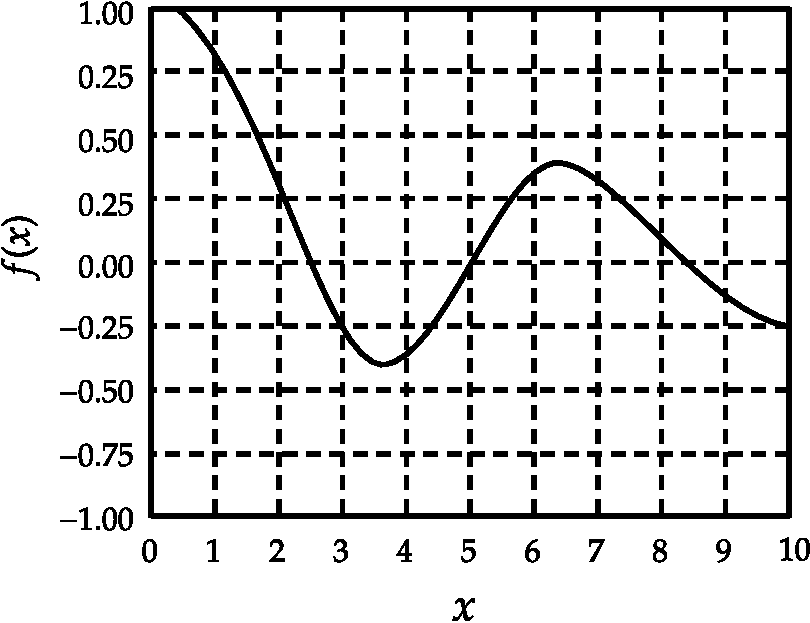
\includegraphics[height=6cm,width=8cm]{diagram-20211005(12)-crop}
	\end{figure}
	\begin{tasks}(2)
		\task[\textbf{A.}]  The Bessel function $J_{0}(x)$
		\task[\textbf{B.}] $\cos x$
		\task[\textbf{C.}] $e^{-x} \cos x$
		\task[\textbf{D.}] $\frac{1}{x} \cos x$
	\end{tasks}
	\item Given that $\sum_{n=0}^{\infty} H_{n}(x) \frac{t^{n}}{n !}=e^{-t^{2}+2 t x}$ the value of $H_{4}(0)$ is
	{\exyear{NET/JRF(JUNE-2013)}}
	\begin{tasks}(4)
		\task[\textbf{A.}] 12
		\task[\textbf{B.}] 6
		\task[\textbf{C.}] 24
		\task[\textbf{D.}] $-6$
	\end{tasks}
	\item   Given $\sum_{n=0}^{\infty} P_{n}(x) t^{n}=\left(1-2 x t+t^{2}\right)^{-1 / 2}$, for $|t|<1$, the value of $P_{5}(-1)$ is
	{\exyear{NET/JRF(JUNE-2014)}}
	\begin{tasks}(4)
		\task[\textbf{A.}] $0.26$
		\task[\textbf{B.}] 1
		\task[\textbf{C.}] $0.5$
		\task[\textbf{D.}] $-1$
	\end{tasks}
	\item The function $f(x)=\sum_{n=0}^{\infty} \frac{(-1)^{n}}{n !(n+1) !}\left(\frac{x}{2}\right)^{2 n+1}$, satisfies the differential equation
	{\exyear{NET/JRF(DEC-2014)}}
	\begin{tasks}(2)
		\task[\textbf{A.}]  $x^{2} \frac{d^{2} f}{d x^{2}}+x \frac{d f}{d x}+\left(x^{2}+1\right) f=0$
		\task[\textbf{B.}]  $x^{2} \frac{d^{2} f}{d x^{2}}+2 x \frac{d f}{d x}+\left(x^{2}-1\right) f=0$
		\task[\textbf{C.}] $x^{2} \frac{d^{2} f}{d x^{2}}+x \frac{d f}{d x}+\left(x^{2}-1\right) f=0$
		\task[\textbf{D.}] $x^{2} \frac{d^{2} f}{d x^{2}}-x \frac{d f}{d x}+\left(x^{2}-1\right) f=0$
	\end{tasks}
	\item
	 The Hermite polynomial $H_{n}(x)$, satisfies the differential equation
	$$
	\frac{d^{2} H_{n}}{d x^{2}}-2 x \frac{d H_{n}}{d x}+2 n H_{n}(x)=0
	$$
	The corresponding generating function $G(t, x)=\sum_{n=0}^{\infty} \frac{1}{n !} H_{n}(x) t^{n}$, satisfies the equation
	{\exyear{NET/JRF(DEC-2015)}}
	\begin{tasks}(2)
		\task[\textbf{A.}] $\frac{\partial^{2} G}{\partial x^{2}}-2 x \frac{\partial G}{\partial x}+2 t \frac{\partial G}{\partial t}=0$
		\task[\textbf{B.}] $\frac{\partial^{2} G}{\partial x^{2}}-2 x \frac{\partial G}{\partial x}-2 t^{2} \frac{\partial G}{\partial t}=0$
		\task[\textbf{C.}] $\frac{\partial^{2} G}{\partial x^{2}}-2 x \frac{\partial G}{\partial x}+2 \frac{\partial G}{\partial t}=0$
		\task[\textbf{D.}]  $\frac{\partial^{2} G}{\partial x^{2}}-2 x \frac{\partial G}{\partial x}+2 \frac{\partial^{2} G}{\partial x \partial t}=0$
	\end{tasks}
	\item A stable asymptotic solution of the equation $x_{n+1}=1+\frac{3}{1+x_{n}}$ is $x=2$. If we take $x_{n}=2+\epsilon_{n}$ and $x_{n+1}=2+\epsilon_{n+1}$, where $\epsilon_{n}$ and $\epsilon_{n+1}$ are both small, the ratio $\frac{\epsilon_{n+1}}{\epsilon_{n}}$ is approximately
	{\exyear{NET/JRF(DEC-2016)}}
	\begin{tasks}(4)
		\task[\textbf{A.}] $-\frac{1}{2}$
		\task[\textbf{B.}] $-\frac{1}{4}$
		\task[\textbf{C.}]  $-\frac{1}{3}$
		\task[\textbf{D.}] $-\frac{2}{3}$
	\end{tasks}
	\item In the function $P_{n}(x) e^{-x^{2}}$ of a real variable $x, P_{n}(x)$ is polynomial of degree $n$. The maximum number of extrema that this function can have is
	{\exyear{NET/JRF(JUNE-2018)}}
	\begin{tasks}(4)
		\task[\textbf{A.}] $n+2$
		\task[\textbf{B.}]  $n-1$
		\task[\textbf{C.}] $n+1$
		\task[\textbf{D.}] $n$
	\end{tasks}
	\item The polynomial $f(x)=1+5 x+3 x^{2}$ is written as linear combination of the Legendre polynomials
	$\left(P_{0}(x)=1, P_{1}(x), P_{2}(x)=\frac{1}{2}\left(3 x^{2}-1\right)\right)$ as $f(x)=\sum_{n} c_{n} P_{n}(x)$. The value of $c_{0}$ is
	{\exyear{NET/JRF(DEC-2018)}}
	\begin{tasks}(4)
		\task[\textbf{A.}] $\frac{1}{4}$
		\task[\textbf{B.}] $\frac{1}{2}$
		\task[\textbf{C.}]  2
		\task[\textbf{D.}]  4
	\end{tasks}
\end{enumerate}
 \colorlet{ocre1}{ocre!70!}
\colorlet{ocrel}{ocre!30!}
\setlength\arrayrulewidth{1pt}
\begin{table}[H]
	\centering
	\arrayrulecolor{ocre}
	\begin{tabular}{|p{1.5cm}|p{1.5cm}||p{1.5cm}|p{1.5cm}|}
		\hline
		\multicolumn{4}{|c|}{\textbf{Answer key}}\\\hline\hline
		\rowcolor{ocrel}Q.No.&Answer&Q.No.&Answer\\\hline
		1&\textbf{D} &2&\textbf{D}\\\hline 
		3&\textbf{A} &4&\textbf{A} \\\hline
		5&\textbf{D} &6&\textbf{C} \\\hline
		7&\textbf{A}&8&\textbf{C}\\\hline
		9&\textbf{A}&10&\textbf{B}\\\hline
		11&\textbf{C} &12&\textbf{B}\\\hline
		13&\textbf{C}&14&\textbf{D}\\\hline
		15&\textbf{C}& &\\\hline
		
	\end{tabular}
\end{table}\newpage 
\begin{abox}
	Problem Set -2
\end{abox}
\begin{enumerate}[label=\color{ocre}\textbf{\arabic*.}]
	\item What is the maximum number of extrema of the function $f(x)=P_{k}(x) e^{-\left(\frac{x^{4}}{4}+\frac{x^{2}}{2}\right)}$, where\\
	$x \in(-\infty, \infty)$ and $P_{k}(x)$ is an arbitrary polynomial of degree $k$ ?
{	\exyear{JEST 2015}}

\begin{tasks}(4)
\task[\textbf{A.}]  $k+2$
\task[\textbf{B.}]$k+6$
\task[\textbf{C.}] $k+3$
\task[\textbf{D.}]$k$
\end{tasks}
\item The Bernoulli polynominals $B_{n}(s)$ are defined by, $\frac{x e^{x s}}{e^{x}-1}=\sum B_{n}(s) \frac{x^{n}}{n !} .$ Which one of the following relations is true?
{\exyear{JEST 2015}}

\begin{tasks}(2)
\task[\textbf{A.}] $\frac{x e^{x(1-s)}}{e^{x}-1}=\sum B_{n}(s) \frac{x^{n}}{(n+1) !}$
\task[\textbf{B.}]$\frac{x e^{x(1-s)}}{e^{x}-1}=\sum B_{n}(s)(-1)^{n} \frac{x^{n}}{(n+1) !}$
\task[\textbf{C.}]$\frac{x e^{x(1-s)}}{e^{x}-1}=\sum B_{n}(-s)(-1)^{n} \frac{x^{n}}{n !}$
\task[\textbf{D.}]$\frac{x e^{x(1-s)}}{e^{x}-1}=\sum B_{n}(s)(-1)^{n} \frac{x^{n}}{n !}$
\end{tasks}
\item For which of the following conditions does the integral $\int_{0}^{1} P_{m}(x) P_{n}(x) d x$ vanish for $m \neq n$, where $P_{m}(x)$ and $P_{n}(x)$ are the Legendre polynomials of order $m$ and $n$ respectively?
{\exyear{JEST 2018}}

\begin{tasks}(2)
\task[\textbf{A.}] all $m, m \neq n$
\task[\textbf{B.}]$m-n$ is an odd integer
\task[\textbf{C.}]$m-n$ is a nonzero even integer
\task[\textbf{D.}]$n=m \pm 1$
\end{tasks}
\item The Euler polynomials are defined by $\frac{2 e^{x s}}{e^{x}+1}=\sum_{n=0}^{\infty} E_{n}(s) \frac{x^{n}}{n !}$What is the value of $E_{5}(2)+E_{5}(3) ?$
{\exyear{JEST 2019}}
\item If $F(x, y)=x^{2}+y^{2}+x y$, its Legendre transformed function $G(u, v)$, upto a multiplicative constant, is
{\exyear{JEST 2018}}

\begin{tasks}(4)
\task[\textbf{A.}] $u^{2}+v^{2}+u v$
\task[\textbf{B.}] $u^{2}+v^{2}-u v$
\task[\textbf{C.}]$u^{2}+v^{2}$
\task[\textbf{D.}]$(u+v)^{2}$
\end{tasks}
\item  Consider a function $f(x)=P_{k}(x) e^{-\left(x^{4}+2 x^{2}\right)}$ in the domain $x \in(-\infty, \infty)$, where $P_{k}$ is any polynomial of degree $k$. What is the maximum possible number of extrema of the function?
{\exyear{JEST 2019}}

\begin{tasks}(4)
\task[\textbf{A.}] $k+3$
\task[\textbf{B.}] $k-3$
\task[\textbf{C.}]$k+2$
\task[\textbf{D.}]$k+1$
\end{tasks}
\end{enumerate}
\colorlet{ocre1}{ocre!70!}
\colorlet{ocrel}{ocre!30!}
\setlength\arrayrulewidth{1pt}
\begin{table}[H]
	\centering
	\arrayrulecolor{ocre}
	\begin{tabular}{|p{1.5cm}|p{1.5cm}||p{1.5cm}|p{1.5cm}|}
		\hline
		\multicolumn{4}{|c|}{\textbf{Answer key}}\\\hline\hline
		\rowcolor{ocrel}Q.No.&Answer&Q.No.&Answer\\\hline
		1&\textbf{C} &2&\textbf{D}\\\hline 
		3&\textbf{A} &4&\textbf{64} \\\hline
		5&\textbf{B} &6&\textbf{D} \\\hline
	
		
	\end{tabular}
\end{table}
\newpage 
\begin{abox}
	Problem Set -3
\end{abox}
\begin{enumerate}[label=\color{ocre}\textbf{\arabic*.}]
\item For real $n$ the cylindrical Bessel function is $J_{n}(x)$ of order $n$ then $J_{n}(x)$ will satisfied differential equation
 \begin{tasks}(1)
	\task[\textbf{a.}]$\frac{d^{2} J_{n}}{d x^{2}}+\frac{1}{x}\left(\frac{d J_{n}}{d x}\right)+\left(1+\frac{n^{2}}{x^{2}}\right) J_{n}=0$
	\task[\textbf{b.}] $\frac{d^{2} J_{n}}{d x^{2}}+\frac{1}{x}\left(\frac{d J_{n}}{d x}\right)+\left(1-\frac{n^{2}}{x^{2}}\right) J_{n}=0$
	\task[\textbf{c.}] $\frac{d^{2} J_{n}}{d x^{2}}+x\left(\frac{d J_{n}}{d x}\right)+\left(1+\frac{n^{2}}{x^{2}}\right) J_{n}=0$
	\task[\textbf{d.}] $\frac{d^{2} J_{n}}{d x^{2}}+x\left(\frac{d J_{n}}{d x}\right)+\left(1-\frac{n^{2}}{x^{2}}\right) J_{n}=0$
\end{tasks}
\begin{answer}
	\begin{align*}
\text{The Bessel function is given by }\frac{d^{2} J_{n}}{d x^{2}}+\frac{1}{x}\left(\frac{d J_{n}}{d x}\right)+\left(1-\frac{n^{2}}{x^{2}}\right) J_{n}=0
	\end{align*}
		So the correct answer is \textbf{Option (b)}
\end{answer}
\item For real $n$ the cylindrical Bessel function is $J_{n}(x)$ of order $n$ then value of $\frac{d J_{0}}{d x}$ is equivalent to 
 \begin{tasks}(4)
	\task[\textbf{a.}] $J_{1}$
	\task[\textbf{b.}]$-J_{1}$
	\task[\textbf{c.}]$2 J_{1}$
	\task[\textbf{d.}]$-2 J_{1}$
\end{tasks}
\begin{answer}
	\begin{align*}
J_{n+1}(x)=-J_{n}^{\prime}(x)+\frac{n}{x} J_{n}\text{. for }n=0, J_{1}=-J_{0}^{\prime}
	\end{align*}
		So the correct answer is \textbf{Option (b)}
\end{answer}
\item  The differential equation $x^{2} \frac{d^{2} y}{d x^{2}}+2 x \frac{d y}{d x}+\left[x^{2}-\lambda\right] y(x)=0$ is spherical Bessel's differential equation of order $n$ then value of $\lambda$ is given by
 \begin{tasks}(4)
	\task[\textbf{a.}]$n$
	\task[\textbf{b.}]$n(n+1)$
	\task[\textbf{c.}] $n(n-1)$
	\task[\textbf{d.}]  $n^{2}$
\end{tasks}
\begin{answer}
	\begin{align*}
\text{Spherical Bessel's differential equation }x^{2} \frac{d^{2} y}{d x^{2}}+2 x \frac{d y}{d x}+\left[x^{2}-n(n+1)\right] y(x)=0
	\end{align*}
		So the correct answer is \textbf{Option (b)}
\end{answer}
\item If $J_{n}(x)$ is spherical Bessel function of order $n$ then $j_{0}^{\prime}(x)$ is equivalent to
 \begin{tasks}(4)
	\task[\textbf{a.}]$j_{1}(x)$
	\task[\textbf{b.}]$-j_{1}(x)$
	\task[\textbf{c.}]$\frac{j_{1}(x)}{2}$
	\task[\textbf{d.}]$-\frac{j_{1}(x)}{2}$
\end{tasks}
\begin{answer}
	\begin{align*}
	\frac{d}{d x}\left(j_{0}(x)\right)&=\frac{d}{d x}\left(\frac{\sin x}{x}\right)=\frac{\cos x}{x}-\frac{\sin x}{x^{2}}=-J_{1}(x)\\
	\text{Where }j_{1}(x)&=-\frac{\cos x}{x}+\frac{\sin x}{x^{2}}
	\end{align*}
	So the correct answer is \textbf{Option (b)}
\end{answer}
\item The solution of the differential equation $x^{2} \frac{d^{2} y}{d x^{2}}+2 x \frac{d y}{d x}+x^{2} y(x)=0$ subjected to the condition is given by $y(0)=1$.
 \begin{tasks}(4)
	\task[\textbf{a.}] $\frac{\sin x}{x}$
	\task[\textbf{b.}] $\frac{\cos x}{x}$
	\task[\textbf{c.}]$\frac{\exp (-i x)}{x}$
	\task[\textbf{d.}] $\frac{\exp i x}{x}$
\end{tasks}
\begin{answer}
	\begin{align*}
 \text{Spherical Bessel's differential equation }&x^{2} \frac{d^{2} y}{d x^{2}}+2 x \frac{d y}{d x}+\left[x^{2}-n(n+1)\right] y(x)=0\\
 \text{ then }x^{2} \frac{d^{2} y}{d x^{2}}+2 x \frac{d y}{d x}+x^{2} y(x)=0 &\text{ is spherical Bessel's differential equation for order}\\
 n&=0\\
	\text{then solution is }J_{0}(x)&=\frac{\sin x}{x}\text{ with boundary condition }y(0)=1.
	\end{align*}
	So the correct answer is \textbf{Option (a)}
\end{answer}
\item $H_{n}(x)$ is Hermite polynomials of order $n$ then $H_{n}(x)=(-1)^{n} f(x) \frac{d^{n}(W(x))}{d x^{n}}$, then $f(x)$ and $W(x)$ are respectively
 \begin{tasks}(1)
	\task[\textbf{a.}]$f(x)=\exp \left(x^{2}\right), W(x)=\exp \left(-x^{2}\right)$
	\task[\textbf{b.}]$f(x)=\exp \left(-x^{2}\right), W=\exp \left(x^{2}\right)$
	\task[\textbf{c.}] $f(x)=W(x)=\exp \left(x^{2}\right)$
	\task[\textbf{d.}] $f(x)=W(x)=\exp \left(-x^{2}\right)$
\end{tasks}
\begin{answer}
	\begin{align*}
	H_{n}(x)&=(-1)^{n} \exp \left(x^{2}\right) \frac{d^{n}\left(\exp \left(-x^{2}\right)\right)}{d x^{n}}\\
	\text{So after comparing }H_{n}(x)&=(-1)^{n} f(x) \frac{d^{n}(W(x))}{d x^{n}}\\
	f(x)&=\exp \left(x^{2}\right), W(x)=\exp \left(-x^{2}\right)
	\end{align*}
		So the correct answer is \textbf{Option (a)}
\end{answer}
\item The solution of differential equation $\frac{d^{2} y}{d x^{2}}-2 x \frac{d y}{d x}+\lambda y(x)=0$ is Hermilte polynomial of order $n$ then value of $\lambda$ is
 \begin{tasks}(4)
	\task[\textbf{a.}]$n$
	\task[\textbf{b.}] $-n$
	\task[\textbf{c.}]$2 n$
	\task[\textbf{d.}] $-2 n$
\end{tasks}
\begin{answer}
	\begin{align*}
	\frac{d^{2} y}{d x^{2}}-2 x \frac{d y}{d x}+2 n y(x)=0\text{ is Hermite differential equation}
	\end{align*}
		So the correct answer is \textbf{Option (c)}
\end{answer}
\item The Rodrigues formula for Laguerre polunomial is given by
 \begin{tasks}(2)
	\task[\textbf{a.}]$L_n(x)=\frac{e^{-x}}{n !}\left(\frac{d}{d x}\right)^{n}\left(x^{n} e^{-x}\right)$
	\task[\textbf{b.}]$L_{n}(x)=\frac{e^{x}}{n !}\left(\frac{d}{d x}\right)^{n}\left(x^{n} e^{x}\right)$
	\task[\textbf{c.}]$L_n(x)=\frac{e^{-x}}{n !}\left(\frac{d}{d x}\right)^{n}\left(x^{n} e^{x}\right)$
	\task[\textbf{d.}] $L_{n}(x)=\frac{e^{x}}{n !}\left(\frac{d}{d x}\right)^{n}\left(x^{n} e^{-x}\right)$
\end{tasks}
\begin{answer}
	\begin{align*}
	L_{n}(x)=\frac{e^{x}}{n !}\left(\frac{d}{d x}\right)^{n}\left(x^{n} e^{-x}\right)
	\end{align*}
		So the correct answer is \textbf{Option (d)}
\end{answer}
\item It is given that operator $x-\frac{d}{d x}=-\exp \left(\frac{x^{2}}{2}\right) \frac{d}{d x} \exp \left(-\frac{x^{2}}{2}\right)$
If then the normalized wave function for harmonic oscillation is $\psi(x)=\left(\pi^{1 / 2} 2^{n}\lfloor n)^{-1 / 2} \exp \left(-\frac{x^{2}}{2}\right) H_{n}(x)\right.$, then $\psi_n(x)$ is equivalent to 
 \begin{tasks}(1)
	\task[\textbf{a.}]$\psi_{n}(x)=\left(\pi^{1 / 2} 2^{n}\lfloor n)^{-1 / 2}\left(x-\frac{d}{d x}\right)^{n} \exp \left(-\frac{x^{2}}{2}\right)\right.$
	\task[\textbf{b.}] $\psi_{n}(x)=\left(\pi^{1 / 2} 2^{n}\lfloor n)^{-1 / 2}\left(x-\frac{d}{d x}\right)^{2 n} \exp \left(\frac{x^{2}}{2}\right)\right.$
	\task[\textbf{c.}] $\psi_{n}(x)=\left(\pi^{1 / 2} 2^{n}\lfloor n)^{-1 / 2}\left(x-\frac{d}{d x}\right)^{n} \exp \left(-x^{2}\right)\right.$
	\task[\textbf{d.}] $\psi_{n}(x)=\left(\pi^{k / 2} 2^{n}\lfloor n)^{-1 / 2}\left(x-\frac{d}{d x}\right)^{2 n} \operatorname{cxp}\left(-x^{2}\right)\right.$
\end{tasks}
\begin{answer}
	\begin{align*}
	H_{n}(x)&=(-1)^{n} \exp \left(x^{2}\right) \frac{d^{n}\left(\exp \left(-x^{2}\right)\right)}{d x^{n}}\\
	x-\frac{d}{d x} &=-\exp \left(\frac{x^{2}}{2}\right) \frac{d}{d x} \exp \left(-\frac{x^{2}}{2}\right) \Rightarrow\left(x-\frac{d}{d x}\right) \exp \left(-\frac{x^{2}}{2}\right) \\ &\left.=-\exp \left(\frac{x^{2}}{2}\right) \frac{d}{d x} \exp \left(-\frac{x^{2}}{2}\right)\right) \exp \left(-\frac{x^{2}}{2}\right)\\
	x \exp \left(-\frac{x^{2}}{2}\right)-\frac{d \exp \left(-\frac{x^{2}}{2}\right)}{d x}&=-\exp \left(\frac{x^{2}}{2}\right) \frac{d}{d x} \exp \left(-x^{2}\right)\\
	\Rightarrow\left(x-\frac{d}{d x}\right) \exp \left(-\frac{x^{2}}{2}\right)&=\exp \left(\frac{x^{2}}{2}\right)\left(-2 x \exp \left(-x^{2}\right)\right)=2 x \exp -\frac{x^{2}}{2}=H_{1}\left(\exp -\frac{x^{2}}{2}\right)\\
	\text{where }2 x&=H_{1}(x)\\
	\text{Similarly }\left(x-\frac{d}{d x}\right)^{n} \exp \left(-\frac{x^{2}}{2}\right)&=H_{n} \exp \left(-\frac{x^{2}}{2}\right)\\
	\psi_{n}(x)&=\left(\pi^{1 / 2} 2^{n}\lfloor n)^{-1 / 2}\left(x-\frac{d}{d x}\right)^{n} \exp \left(-\frac{x^{2}}{-2}\right)\right.
	\end{align*}
	So the correct answer is \textbf{Option (a)}
\end{answer}
\item The solution of differential equation $x \frac{d^{2} y}{d x^{2}}+(1-x) \frac{d y}{d x}+\lambda y(x)=0$ is Laguerre polynomials of order $n$ then value of $\lambda$ is
 \begin{tasks}(4)
	\task[\textbf{a.}]$n$
	\task[\textbf{b.}]$-n$
	\task[\textbf{c.}] $2 n$
	\task[\textbf{d.}] $-2 n$
\end{tasks}
\begin{answer}
	\begin{align*}
	x \frac{d^{2} y}{d x^{2}}+(1-x) \frac{d y}{d x}+n y(x)=0\text{ is Laguerre differential equation.}
	\end{align*}
	So the correct answer is \textbf{Option (a)}
\end{answer}
\item The generating function $F(x, t)=\sum_{n=0}^{\infty} P_{n}(x) t^{n}$ for the Legendre polynomials $P_{n}(x)$ is $F(x, t)=\left(1-2 x t+t^{2}\right)^{-1 / 2}$. The value of $P_{2}(-1)$ is
 \begin{tasks}(4)
	\task[\textbf{a.}]$5 / 2$
	\task[\textbf{b.}]$3 / 2$
	\task[\textbf{c.}] $+1$
	\task[\textbf{d.}] $-1$
\end{tasks}
\begin{answer}
	\begin{align*}
	\text{The generating function for Legendre polynomial is }F(x, t)&=\left(1-2 x t+t^{2}\right)^{-1 / 2}.\text{ Thus}\\P_{2}(x)=\frac{1}{2}\left(3 x^{2}-1\right) \Rightarrow P_{2}(-1)=\frac{1}{2}(3-1)=1
	\end{align*}
		So the correct answer is \textbf{Option (c)}
\end{answer}
\item If we observe plot of Bessel functions $J_{0}(x), J_{1}(x)$, and $J_{2}(x)$ we find their maxima at $x_{0}, x_{1}$ and $x_{2}$ respectively. Then which of the following is true
 \begin{tasks}(2)
	\task[\textbf{a.}]$x_{0}<x_{1}<x_{2}$
	\task[\textbf{b.}]$x_{0}>x_{1}>x_{2}$
	\task[\textbf{c.}]$x_{0}<x_{1}=x_{2}$
	\task[\textbf{d.}] $x_{0}=x_{1}<x_{2}$
\end{tasks}
\begin{answer}
	So the correct answer is \textbf{Option (a)}
\end{answer}
\item Which one of the following is correctly matched?\\
\begin{figure}[H]
	\centering
	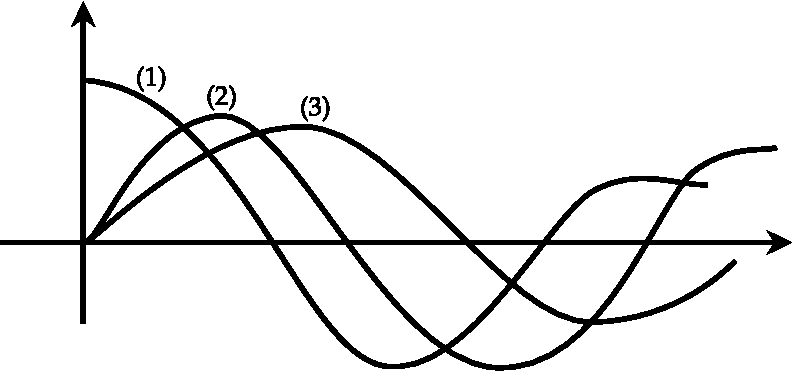
\includegraphics[height=3.5cm,width=6.5cm]{SF-01}
\end{figure}
 \begin{tasks}(2)
	\task[\textbf{a.}](1) $J_{0}$,
	(2) $J_{2}$, (3) $J_{1}$
	\task[\textbf{b.}]$(1) J_{0}$,
	(2) $J_{1}, \quad(3) J_{2}$
	\task[\textbf{c.}](1) $J_{2}$,
	(2) $J_{1}$,
	(3) $J_{0}$
	\task[\textbf{d.}] None of the above
\end{tasks}
\begin{answer}
	So the correct answer is \textbf{Option (b)}
\end{answer}
\item If the generating function of Legendre polynomial is $\frac{1}{\sqrt{1-6 t+t^{2}}}$, then coefficient of $t^{2}$ is
 \begin{tasks}(4)
	\task[\textbf{a.}] 11
	\task[\textbf{b.}]$-11$
	\task[\textbf{c.}]13
	\task[\textbf{d.}] $-13$
\end{tasks}
\begin{answer}
	\begin{align*}
	\intertext{The generating function for the polynomial solutions of the Legendre ODE is given by}
	g(x, t)&=\frac{1}{\sqrt{1-2 x t+t^{2}}}=\sum_{n=0}^{\infty} P_{n}(x) t^{n}\\
	\text{Thus }x&=3\text{ and }n=2.\\
	P_{2}(x)&=\frac{1}{2}\left(3 x^{2}-1\right) \Rightarrow P_{2}(3)=\frac{1}{2}\left(3 \times 3^{2}-1\right)=13
	\end{align*}
		So the correct answer is \textbf{Option (c)}
\end{answer}
\item Which of the following relation is true for Bessel's differential equation?
 \begin{tasks}(2)
	\task[\textbf{a.}]$J_{0}^{\prime}(x)=J_{1}(x)$
	\task[\textbf{b.}]$J_{0}^{\prime}(x)=-J_{2}(x)$
	\task[\textbf{c.}]$J_{0}^{\prime}(x)=J_{2}(x)$
	\task[\textbf{d.}] $J_{0}^{\prime}(x)=-J_{1}(x)$
\end{tasks}
\begin{answer}
	So the correct answer is \textbf{Option (d)}
\end{answer}
\end{enumerate}